\documentclass[a4paper]{article}
\usepackage[utf8]{inputenc}
\usepackage[spanish, es-tabla]{babel}

\usepackage[a4paper, footnotesep = 1cm, width=18cm, left=2cm, top=2.5cm, height=25cm, textwidth=18cm, textheight=25cm]{geometry}
%\geometry{showframe}

\usepackage{amsmath}
\usepackage{amsfonts}
\usepackage{amssymb}
\usepackage{float}
\usepackage{graphicx}
\usepackage{caption}
\usepackage{subcaption}
\usepackage{multicol}
\usepackage{multirow}
\setlength{\doublerulesep}{\arrayrulewidth}

\usepackage{hyperref}
\hypersetup{
    colorlinks=true,
    linkcolor=blue,
    filecolor=magenta,      
    urlcolor=blue,
    citecolor=blue,    
}

\newcommand{\quotes}[1]{``#1''}
\usepackage{array}
\newcolumntype{C}[1]{>{\centering\let\newline\\\arraybackslash\hspace{0pt}}m{#1}}
\usepackage[american]{circuitikz}
\usepackage{fancyhdr}
\usepackage{units} 

\pagestyle{fancy}
\fancyhf{}
\lhead{22.11 Electrónica I}
\rhead{Mechoulam, Lambertucci, Rodriguez, Londero}
\rfoot{Página \thepage}

\begin{document}

%%%%%%%%%%%%%%%%%%%%%%%%%
%		Caratula		%
%%%%%%%%%%%%%%%%%%%%%%%%%

\begin{titlepage}
\newcommand{\HRule}{\rule{\linewidth}{0.5mm}}
\center
\mbox{\textsc{\LARGE \bfseries {Instituto Tecnológico de Buenos Aires}}}\\[1.5cm]
\textsc{\Large 22.11 Electrónica I}\\[0.5cm]


\HRule \\[0.6cm]
{ \Huge \bfseries Trabajo práctico N$^{\circ}$1}\\[0.4cm] 
\HRule \\[1.5cm]


{\large

\emph{Grupo 3}\\
\vspace{3px}

\begin{tabular}{lr} 	
\textsc{Mechoulam}, Alan  &  58438\\
\textsc{Lambertucci}, Guido Enrique  & 58009 \\
\textsc{Rodriguez Turco}, Martín Sebastian  & 56629 \\
\textsc{Londero Bonaparte}, Tomás Guillermo  & 58150 \\
\end{tabular}

\vspace{20px}

\emph{Profesores}\\
Alcocer, Fernando\\
Oreglia, Eduardo Victor\\
Gardella, Pablo Jesús\\
\vspace{3px}
%\textsc{} \\	

\vspace{100px}

\begin{tabular}{ll}

Presentado: & 24/09/19\\

\end{tabular}

}

\vfill

\end{titlepage}


%%%%%%%%%%%%%%%%%%%%%
%		Indice		%
%%%%%%%%%%%%%%%%%%%%%

\tableofcontents
\newpage

%%%%%%%%%%%%%%%%%%%%%
%		Informe		%
%%%%%%%%%%%%%%%%%%%%%
\section{Introducción}
En el siguiente informe se busca analizar, desarrollar y confeccionar algún circuito estudiado a lo largo del cuatrimestre. Se destaca la existencia de una dificultad adicional, la cual se basa en el método mediante el cual se fueron adquiriendo los componentes. Estos fueron subastados durante la cursada, entre los diversos grupos. De esta forma, se condiciona el circuito final, ya que no se pudieron elegir libremente los componentes a utilizar.

\section{Desarrollo}

\subsection{Componentes dispuestos}
El presente grupo se valió de los siguientes componentes:
\begin{itemize}
	\item Dos pares de resistencias de $6.8 \ K\omega$ y de $680 \ K\omega$.
	\item Un transistor BJT NPN. 
	\item Un diodo 1N4148.
	\item Un JFET.
	\item Un par Darlington NPN.
	\item Una placa de 5x5.
\end{itemize}

\subsection{Circuitos considerados}
Como primer opción se consideró utilizar el par Darlington y mediante el uso de las resistencias, configurarlo de forma tal tal que este quede compensado. Una alternativa a lo previamente mencionado es el uso de JFET como una fuente de corriente, con el mismo objetivo que se mencionó anteriormente, ya que colocar una fuente de corriente es la solución optima a la compensación.

\begin{figure}[H]
\centering
\begin{subfigure}{.4\textwidth}
\centering
	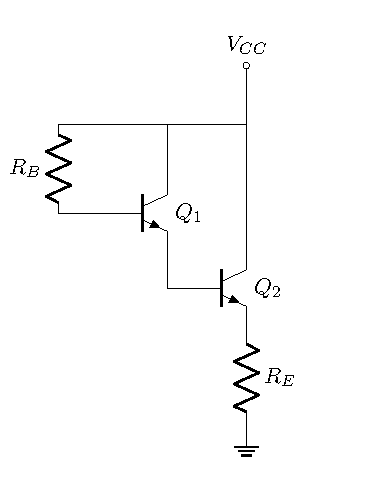
\includegraphics[width=0.6\textwidth, page=1]{Imagenes/ParDarlington.pdf}
	\caption{Par Darlington.}
	\label{fig:pardar1}
\end{subfigure}
\begin{subfigure}{.5\textwidth}
\centering
	\includegraphics[width=0.5\textwidth, page=2]{Imagenes/ParDarlington.pdf}
	\caption{Par Darlington compensado con $R$.}
	\label{fig:pardar2}
\end{subfigure}

\begin{subfigure}{.5\textwidth}
\centering
	\includegraphics[width=0.5\textwidth, page=3]{Imagenes/ParDarlington.pdf}
	\label{fig:pardar3}
	\caption{Par Darlington compensado con fuente de corriente.}
\end{subfigure}
\end{figure}

\section{Conclusiones}
	
\end{document}